\documentclass[12pt]{article}
\usepackage{setspace}
\usepackage{latexsym}
\usepackage{amssymb,amsmath}
\usepackage[pdftex]{graphics}
\usepackage{graphicx}
\usepackage{amsthm}


\topmargin = -0.5in \textwidth=6.5in \textheight=9in

\oddsidemargin = 0in \evensidemargin = 0in

\DeclareMathSizes{12}{10}{7}{5}
\newcommand{\bphi}{\bar{\phi}}
\newcommand{\bw}{\bar{w}}
\newcommand{\bv}{\bar{v}}
\newcommand{\bF}{\bar{F}}
\newcommand{\bg}{\bar{g}}
\newcommand{\be}{\bar{\eta}}
\newcommand{\br}{\bar{\rho}}
\newcommand{\bmu}{\bar{\mu}}
\newcommand{\bx}{\bar{x}}
\newcommand{\bS}{\bar{S}}
\newcommand{\bT}{\bar{T}}
\newcommand{\sq}{\sqrt{2}}
\newcommand{\hr}{\hat{r}}
\newcommand{\hy}{\hat{y}}
\newcommand{\hY}{\hat{Y}}
\newcommand{\tx}{\tilde{x}}
\newcommand{\tW}{\tilde{W}}
\newcommand{\tb}{\tilde{b}}
\newcommand{\tg}{\tilde{g}}
\newcommand{\tz}{\tilde{z}}
\newcommand{\eps}{\epsilon}
\newcommand{\teps}{\tilde{\epsilon}}
\newcommand{\tS}{\tilde{S}}
\newcommand{\tA}{\tilde{A}}
\newcommand{\tsigma}{\tilde{\sigma}}
\newcommand{\ulq}{\underline{q}}
\newcommand{\olq}{\overline{q}}
\newcommand{\ulr}{\underline{r}}
\newcommand{\olr}{\overline{r}}
\newcommand{\Exp}{\ProbOpr{E}}
%\usepackage{graphicx}
%\usepackage{amsmath,amsfonts,amssymb,amsopn,amsbsy,amsthm}
%\usepackage{dsfont,bm,bbm,times,url,verbatim,epstopdf,xspace}
%\usepackage[capitalize]{cleveref}
%\usepackage{placeins}
%\usepackage{amssymb,amsthm}
%\usepackage{bbm,epstopdf}
%\usepackage[group-separator={,}]{siunitx}
%\usepackage[export]{adjustbox}
%\usepackage{hhline}
%\usepackage[hypertexnames=false]{hyperref}
% for footnotes without markers
%\newcommand\blfootnote[1]{%
%  \begingroup
%  \renewcommand\thefootnote{}\footnote{#1}%
%  \addtocounter{footnote}{-1}%
%  \endgroup
%}

% New commands added from Nystrom notes.
\newcommand{\Nystrom}{Nystr\"{o}m }
\newcommand{\NystromNS}{Nystr\"{o}m} % NS means ``no space''
\newcommand{\NystromCaps}{NYSTR\"{O}M }
\newcommand{\NystromCapsNS}{NYSTR\"{O}M} % NS means ``no space''
\newcommand{\Ap}{A^\perp}
\newcommand{\mua}{\mu_A}
\newcommand{\muap}{\mu_{\Ap}}
\newcommand{\bphi}{\bar{\phi}}
\newcommand{\by}{\bar{y}}
%\newcommand{\bw}{\bar{w}}
%\newcommand{\bv}{\bar{v}}
%\newcommand{\bF}{\bar{F}}
%\newcommand{\bg}{\bar{g}}
%\newcommand{\be}{\bar{\eta}}
%\newcommand{\br}{\bar{\rho}}
%\newcommand{\bU}{\bar{U}}
%\newcommand{\bV}{\bar{V}}
%\newcommand{\bLam}{\bar{\Lambda}}
%\newcommand{\bL}{\bar{L}}
\newcommand{\hx}{\hat{x}}
\newcommand{\hb}{\hat{b}}
%\newcommand{\hX}{\hat{X}}
%\newcommand{\hY}{\hat{Y}}
\newcommand{\hp}{\hat{\phi}}
\newcommand{\hK}{\hat{K}}
%\newcommand{\tp}{\tilde{\phi}}
\newcommand{\tk}{\tilde{k}}
%\newcommand{\tC}{\tilde{C}}
\newcommand{\eps}{\epsilon}
\newcommand{\teps}{\tilde{\epsilon}}
\newcommand{\tS}{\tilde{S}}
\newcommand{\tK}{\tilde{K}}
\newcommand{\tA}{\tilde{A}}
\newcommand{\tf}{\tilde{f}}
\newcommand{\tsigma}{\tilde{\sigma}}
\newcommand{\tgamma}{\tilde{\gamma}}
\newcommand{\tlambda}{\tilde{\lambda}}
\newcommand{\hcR}{\hat{\cR}}
\newcommand{\id}{I}
\newcommand{\ulq}{\underline{q}}
\newcommand{\olq}{\overline{q}}
\newcommand*{\QED}{\hfill\ensuremath{\square}}

\newcommand*\conj[1]{\overline{#1}}

% note: I removed the package amsthm because it defines "proof", which is already defined in jmlr2e package
\newcommand{\ie}{i.e.}
\newcommand{\eg}{e.g.}
\newcommand{\etal}{et al.}
\def\ddefloop#1{\ifx\ddefloop#1\else\ddef{#1}\expandafter\ddefloop\fi}
%
%% \bbA, \bbB, ...
\def\ddef#1{\expandafter\def\csname bb#1\endcsname{\ensuremath{\mathbb{#1}}}}
\ddefloop ABCDEFGHIJKLMNOPQRSTUVWXYZ\ddefloop
%
%% \bfA, \bfB, ...
%\def\ddef#1{\expandafter\def\csname bf#1\endcsname{\ensuremath{\mathbf{#1}}}}
%\ddefloop ABCDEFGHIJKLMNOPQRSTUVWXYZabcdefghijklmnopqrstuvwxyz\ddefloop
%
%% \bfalpha, \bfbeta, ...,  \bfGamma, \bfDelta, ...,
%\def\ddef#1{\expandafter\def\csname bf#1\endcsname{\ensuremath{\pmb{\csname #1\endcsname}}}}
%\ddefloop {alpha}{beta}{gamma}{delta}{epsilon}{varepsilon}{zeta}{eta}{theta}{vartheta}{iota}{kappa}{lambda}{mu}{nu}{xi}{pi}{varpi}{rho}{varrho}{sigma}{varsigma}{tau}{upsilon}{phi}{varphi}{chi}{psi}{omega}{Gamma}{Delta}{Theta}{Lambda}{Xi}{Pi}{Sigma}{varSigma}{Upsilon}{Phi}{Psi}{Omega}{ell}\ddefloop
%
%% \cA, \cB, ...
\def\ddef#1{\expandafter\def\csname c#1\endcsname{\ensuremath{\mathcal{#1}}}}
\ddefloop ABCDEFGHIJKLMNOPQRSTUVWXYZ\ddefloop
%
%% \mbf0, \mbf1, ...
%\newcommand\mbf{\ensuremath{\mathbf}}
%
%\DeclareMathOperator*{\argmin}{arg\,min}
%\DeclareMathOperator*{\argmax}{arg\,max}
%
%\newcommand\parens[1]{(#1)}
\newcommand\norm[1]{\|#1\|}
%\newcommand\braces[1]{\{#1\}}
%\newcommand\brackets[1]{[#1]}
%\newcommand\ceil[1]{\lceil#1\rceil}
%\newcommand\abs[1]{|#1|}
%\newcommand\ind[1]{\ensuremath{\mathds{1}\{#1\}}}
\newcommand\dotp[1]{\langle #1 \rangle}
%\newcommand\Parens[1]{\left(#1\right)}
%\newcommand\Norm[1]{\left\|#1\right\|}
%\newcommand\Braces[1]{\left\{#1\right\}}
%\newcommand\Brackets[1]{\left[#1\right]}
%\newcommand\Ceil[1]{\left\lceil#1\right\rceil}
%\newcommand\Abs[1]{\left|#1\right|}
%\newcommand\Ind[1]{\mathds{1}\left\{#1\right\}}
\newcommand\Dotp[1]{\left\langle#1\right\rangle}
%
\newcommand{\RR}{\ensuremath{\bbR}} %real numbers
\newcommand{\Nat}{\ensuremath{\bbN}} %natural numbers 
\newcommand{\CC}{\ensuremath{\bbC}} %complex numbers
%
%\newcommand{\risk}{\ensuremath{R}} % risk
%\newcommand{\loss}{\ensuremath{\ell}} % loss
%\newcommand{\logloss}{\ensuremath{\ell_{\operatorname{log}}}} % logistic loss
%
%\newcommand{\rfm}{\ensuremath{z}} % (random) feature map
%\newcommand{\kfm}{\ensuremath{\phi}} % kernel feature map
%\newcommand{\kernel}{\ensuremath{K}} % kernel function
%
%%\setlength{\marginparwidth}{25mm}
%\usepackage[textsize=tiny]{todonotes}
%%\usepackage[disable]{todonotes}
%\newcommand{\djh}[2][]{\todo[color=red!20!white,#1]{DH: #2}}
%\newcommand{\avner}[2][]{\todo[color=red!20!white,#1]{AM: #2}}
\newcommand\todo[1]{\textcolor{red}{#1}}
\newcommand\avner[1]{\textcolor{red}{AM: #1}}
\newcommand\tri[1]{\textcolor{red}{TD: #1}}
\newcommand\jian[1]{\textcolor{red}{JZ: #1}}
%
%\newcommand{\numtr}{\ensuremath{n_{\operatorname{tr}}}}
%\newcommand{\numho}{\ensuremath{n_{\operatorname{ho}}}}
%\newcommand{\numte}{\ensuremath{n_{\operatorname{te}}}}
%
%\usepackage{tabularx}
%\newcolumntype{Y}{>{\centering\arraybackslash}X}
%\usepackage{multirow}
%
%\usepackage{algorithm}
%\usepackage{algorithmic}
%\usepackage{pdflscape}
%
%% define vector and matrix symbols
%\newcommand{\vct}[1]{\boldsymbol{#1}} % vector
%\newcommand{\mat}[1]{\boldsymbol{#1}} % matrix
%\newcommand{\cst}[1]{\mathsf{#1}}  % constant
%
%%%%% Special math symbols
%\newcommand{\field}[1]{\mathbb{#1}}
%\newcommand{\R}{\field{R}} % real domain
%\newcommand{\C}{\field{C}} % complex domain
%\newcommand{\F}{\field{F}} % functional domain
%%\newcommand{\T}{^{\top}\!\!} % transpose
%\newcommand{\T}{^{\textrm T}} % transpose
%
%%% operator in linear algebra, functional analysis
%\newcommand{\inner}[2]{#1\cdot #2}
%%\newcommand{\norm}[1]{\|#1\|}
%\newcommand{\twonorm}[1]{\left\|#1\right\|_2^2}
%\newcommand{\onenorm}[1]{\|#1\|_1}
%\newcommand{\Map}[1]{\mathcal{#1}}  % operator in functions, maps such as M: domain1 --> domain 2
%
%% operator in probability: expectation, covariance, 
\newcommand{\E}{\mathbb{E}} % Expectation symbol (ADDED BY TRI)
\newcommand{\Prob}{\mathbb{P}}
\newcommand{\ProbOpr}[1]{\mathbb{#1}}
%% independence
%\newcommand\independent{\protect\mathpalette{\protect\independenT}{\perp}}
%\def\independenT#1#2{\mathrel{\rlap{$#1#2$}\mkern2mu{#1#2}}}
%%\newcommand{\ind}[2]{{#1} \independent{#2}}
%\newcommand{\cind}[3]{{#1} \independent{#2}\,|\,#3} % conditional independence
\newcommand{\expect}[2]{%
\ifthenelse{\equal{#2}{}}{\ProbOpr{E}_{#1}}
{\ifthenelse{\equal{#1}{}}{\ProbOpr{E}\left[#2\right]}{\ProbOpr{E}_{#1}\left[#2\right]}}} % Expectation: syntax: E{1}{2} = E_1[2], E{}{2}=E[2], E{1}{} = E_1
%\newcommand{\var}[2]{%
%\ifthenelse{\equal{#2}{}}{\ProbOpr{VAR}_{#1}}
%{\ifthenelse{\equal{#1}{}}{\ProbOpr{VAR}\left[#2\right]}{\ProbOpr{VAR}_{#1}\left[#2\right]}}} % Expectation: syntax: V{1}{2} = V_1[2], V{}{2}=V[2], V{1}{} = V_1
%\newcommand{\cndexp}[2]{\ProbOpr{E}\,[ #1\,|\,#2\,]}  % conditional expectation
%
%% operator in optimization
%%\DeclareMathOperator{\argmax}{arg\,max}
%%\DeclareMathOperator{\argmin}{arg\,min}
%
%% special functions
%\newcommand{\trace}[1]{\operatornamewithlimits{tr}\left\{#1\right\}}
\newcommand{\diag}{\operatornamewithlimits{diag}}
%\newcommand{\sign}{\operatornamewithlimits{sign}}
%\newcommand{\const}{\operatornamewithlimits{const}}
%
%% special display
%\newcommand{\parde}[2]{\frac{\partial #1}{\partial  #2}}
%
%
%% environment
%\newtheorem{thm}{Theorem}
\newtheorem{theorem}{Theorem}
\newtheorem{definition}{Definition}
\newtheorem{lemma}[theorem]{Lemma}
\newtheorem{conjecture}[theorem]{Conjecture}
\newtheorem{proposition}[theorem]{Proposition}
\newtheorem{claim}{Claim}
\newtheorem{corollary}{Corollary}[theorem]

%\newtheorem{thm}{Theorem}
%\newtheorem{theorem}{Theorem}
%\newtheorem{claimcor}{Corollary}[claim]
%\newtheorem{lemma}{Lemma}[theorem]



%% DPP symbols
%\newcommand{\Xt}{{\mathcal{X}_{(t)}}} % X_t
%\newcommand{\Yt}{{Y_{(t)}}} % Y_t
%\newcommand{\Ystart}{{Y^{\star}_{(t)}}} % Y*_t
%\newcommand{\ground}{{\mathcal{Y}}} % ground set
%\newcommand{\groundX}{{\mathcal{X}}} % ground set
%
%
%
%% shorthand
%\newcommand{\vtheta}{\vct{\theta}}
%\newcommand{\vmu}{\vct{\mu}}
%\newcommand{\valpha}{\vct{\alpha}}
%\newcommand{\vc}{\vct{c}}
%\newcommand{\vp}{\vct{p}}
%\newcommand{\vq}{\vct{q}}
%\newcommand{\vx}{{\vct{x}}}
%\newcommand{\vy}{\vct{y}}
%\newcommand{\vz}{{\vct{z}}}
%\newcommand{\vu}{\vct{u}}
%\newcommand{\vo}{{\vct{o}}}
%\newcommand{\va}{\vct{a}}
%\newcommand{\vb}{\vct{b}}
%\newcommand{\vr}{\vct{r}}
%\newcommand{\vt}{\vct{t}}
%\newcommand{\vs}{\vct{s}}
%\newcommand{\vv}{\vct{v}}
%\newcommand{\vw}{\vct{w}}
%\newcommand{\ones}{\vct{1}}
%\newcommand{\mU}{\mat{U}}
%\newcommand{\mA}{\mat{A}}
%\newcommand{\mB}{\mat{B}}
%\newcommand{\mC}{\mat{C}}
%\newcommand{\mW}{\mat{W}}
%\newcommand{\mH}{\mat{H}}
%\newcommand{\mS}{\mat{S}}
%\newcommand{\mJ}{\mat{J}}
%\newcommand{\mM}{\mat{M}}
%\newcommand{\mT}{\mat{T}}
%\newcommand{\mZ}{\mat{Z}}
%\newcommand{\mO}{\mat{O}}
%\newcommand{\mY}{\mat{Y}}
%%\newcommand{\cN}{\cst{N}}
%%\newcommand{\cQ}{\cst{Q}}
%%\newcommand{\cD}{\cst{D}}
%%\newcommand{\cL}{\cst{L}}
%%\newcommand{\cK}{\cst{K}}
%%\newcommand{\cH}{\cst{H}}
%\newcommand{\sQ}{\mathcal{Q}}
%\newcommand{\sS}{\mathcal{S}}
%\newcommand{\mL}{\mat{L}}
%\newcommand{\mI}{\mat{I}}
%\newcommand{\mK}{\mat{K}}
%\newcommand{\mSigma}{\mat{\Sigma}}
%\newcommand{\sF}{\mathcal{F}}
%\newcommand{\vzero}{\vct{0}}
%\newcommand{\vf}{\vct{f}}
%\newcommand{\vF}{\vct{F}}
%\newcommand{\vP}{\vct{P}}
%
%
%\newcommand{\vh}{\vct{h}}
%\newcommand{\vg}{\vct{g}}
%\newcommand{\vphi}{\vct{\phi}}
%\newcommand{\vpsi}{\vct{\psi}}
%\newcommand{\vdelta}{\vct{\delta}}
%\newcommand{\vomega}{\vct{\omega}}
%\newcommand{\mOmega}{\mat{\Omega}}
%
%% 
%\newcommand{\nx}{\tilde{x}}
%\newcommand{\vnx}{{\tilde{\vx}}}
%\newcommand{\vnz}{{\tilde{\vz}}}
%%\newcommand{\deltavx}{(\vnx-\vx)}
%\newcommand{\deltavx}{\delta_\vx}
%\newcommand{\vmx}{\bar{\vx}}
%\newcommand{\vmz}{\bar{\vz}}
%\newcommand{\sigmax}{\mSigma_{\vx}}
%\newcommand{\sigmaz}{\mSigma_{\vz}}
%\newcommand{\no}{\tilde{o}}
%\newcommand{\vno}{{\tilde{\vo}}}
%\newcommand{\nell}{\tilde{\ell}}
%\newcommand{\jacob}{\mat{J}}
%\newcommand{\hess}{\mat{H}}
%\newcommand{\mloss}{\hat{\ell}}
%\newcommand{\vDD}{\vct{\Delta}}
%%
%\newcommand{\eat}[1]{}
%
%\newcommand{\FS}[1]{{\color{blue}FS:#1}}
%
%\newcommand\id{\ensuremath{\mathbbm{1}}}
%\newcommand*{\QED}{\hfill\ensuremath{\square}}
\newcommand{\defeq}{:=}
\newcommand{\eqdef}{=:}
\newcommand{\var}{{\rm Var}} % Variance
\providecommand{\tr}{\mathop{\rm tr}}
\begin{document}


\title{Low-Precision Random Fourier Features (LP-RFF)}
\author{Avner May}
\onehalfspacing
\maketitle

\section{Spark notes}
In this work we will analyze, empirically and theoretically, the performance of low-precision random features.  Specifically, we will consider quantizing the features of the form $z_i(x) = \sqrt{\frac{2}{m}} \cos(w_i^Tx+b_i)$ into $b$-bits, through some form of quantization scheme (simplest: random rounding).  We will generally assume we are using the $(\delta,b)$ low-precision format from the HALP paper, where the numbers representable are $\delta\cdot (-2^{b-1},\ldots,-1,0,1,2^{b-1}-1)$.  To simplify analysis, and make the domain of representable values symmetric around 0, we will often consider the shifted domain $\delta \cdot (-2^{b-1} + \frac{1}{2}, -2^{b-1} + \frac{3}{2},\ldots, -\frac{1}{2},\frac{1}{2},\ldots, 2^{b-1}-\frac{3}{2}, 2^{b-1}-\frac{1}{2})$.  \\

\noindent Main questions
\begin{itemize}
	\item Can we analyze the variance of these low-precision features, in their approximation of the kernel?  Concentration inequalities?
	\item Can we analyze the generalization performance of these features?
	\item How should model training be performed on top of these low-precision features? Can we train in low-precision, and if so, what would the effects of such a training scheme be on the performance of the model?
\end{itemize}

I will now present some initial theoretical results.  In the section below, assume that $Q_b:\RR\rightarrow\RR$ is a random quantization function which quantizes the interval $[-\sq,\sq]$ into $b$ bits, representing the values $\frac{2\sq}{2^b-1} \cdot (-2^{b-1} + \frac{1}{2}, -2^{b-1} + \frac{3}{2},\ldots, -\frac{1}{2},\frac{1}{2},\ldots, 2^{b-1}-\frac{3}{2}, 2^{b-1}-\frac{1}{2})$, with the property that $\expect{}{Q_b(z)} = z \; \forall b,z$.  Given this quantization, we will define a ``quantization interval'' to be the set of points between two consecutive quantized values.
For $z\in [-\sq,\sq]$, let $\ulq(z)$ be the ``bottom'' of the quantization interval containing $z$, let $\olq(z)$ denote the ``top'' of this interval.

\subsection{Initial Theoretical Results}
\begin{itemize}
%	\item \noindent\textbf{Definitions}: For $z \in [a,c]$, let $X_z^{a,c}$ be the random variable which with probability $\frac{z-a}{c-a}$ equals $c-z$, and with probability $\frac{c-z}{c-a}$ equals $a-z$. Furthermore, let $Q^{a,c}(z) = z + X_z^{a,c} \in \{a,c\}$ be the ``quantized'' version of $z$, corresponding to randomized rounding to $a$ or $c$.
	\item \textbf{Proposition 1} (Variance of LP-RFF):  For $x,y\in\cX$ fixed, let $S=Z_x Z_y$, $T = Q_b(Z_x)Q_b(Z_y)$, with $\expect{}{S}=\expect{}{T} = k(x,y)$, and $\expect{S}{(S-k(x,y))^2} = \sigma^2$, $\expect{Q_b}{(Q_b(z_x)Q_b(z_y)-z_x z_y)^2} = \tsigma_b^2$, for $z_x,z_y$ fixed.  Now, let $(S_1,\ldots,S_n)$, $(T_1,\ldots,T_n)$ be a random sequence of i.i.d. draws from $S$ and $T$ respectively.  Define $\bar{S}_n = \frac{1}{n}\sum_{i=1}^n S_i$, and $\bar{T}_n =  \frac{1}{n}\sum_{i=1}^n T_i$, to be the empirical mean of these draws.  It follows that $\expect{}{\bS_n} = \expect{}{\bT_n} = k(x,y)$, and that
	$\var{}{\bS_n} = \frac{\sigma^2}{n}$, and $\var{}{\bT_n} = \frac{\sigma^2 + \tsigma_b^2}{n}$.
	Furthermore, $\tsigma_b^2 = (z_x-\ulq(z_x))(\olq(z_x)-z_x)(z_y-\ulq(z_y))(\olq(z_y)-z_y) \leq \frac{1}{4}(\frac{2\sq}{2^b-1})^2= \frac{2}{(2^b-1)^2}$.
	
	
%	$r = \frac{2\sq}{2^b-1}$. 
%	Thus, from Lemma 1 (see footnote) the quantization error $\tsigma_b^2 \leq r^2/4 = \frac{2}{(2^b-1)^2}$. 
	\item \textbf{Proposition 2} (Concentration bounds for LP-RFF): For a fixed $x,y\in\cX$, let $S$ be any random variable with the property that $\expect{}{S} = k(x,y)$, and $S \in [-2,2]$.\footnote{$S=Q_b(\sq\cos(w^Tx+b))Q_b(\sq\cos(w^Ty+b))$ satisfies these conditions.}  Let $(S_1,\ldots,S_n)$, be a random sequence of i.i.d. draws from $S$, and let $\bS_n = \frac{1}{n}\sum_{i=1}^n S_i$ be the empirical mean of this sequence.  Then, it follows directly from Hoeffding's inequality that $\Prob{\big[|\bS_n - k(x,y)| \geq \epsilon\big]} \leq 2\exp(-n\eps^2/8)$.
	\item \textbf{Proposition 3} (Generalization bounds for LP-RFF: extending Theorem 1 of $[4]$ to LP-RFF):
	Let $\phi:\cX\times\Omega\rightarrow\RR$ be a set of feature functions such that $\sup_{x,w}|\phi(x;w)| \leq 1$. Assume there exists a family of deterministic quantization functions $\{Q_{\theta}:\RR\rightarrow\RR \;|\; \theta\in\Theta \}$, parameterized by some parameter $\theta\in\Theta$.  Let $p_{\Theta}$ be a probability distribution over $\Theta$, $p_{\Omega}$ be a probability distribution over $\Omega$, and define $p(w,\theta) = p_{\Omega}(w)p_{\Theta}(\theta)$.
	Define the quantized feature functions as $\phi'(x;w,\theta) = Q_{\theta}(\phi(x;w))$, and define
	$$\cF_p = \bigg\{f(x) = \int_{\Omega\times\Theta} \alpha(w,\theta) \phi'(x;w,\theta)dwd\theta \;\;\bigg|\;\; |\alpha(w,\theta)| \leq Cp(w,\theta)\bigg\}.$$
	Suppose the cost function $c(y,y') = c(yy')$, with $c(yy')$ $L$-Lipschitz.  Then for any $\delta > 0$, if the training data $\{x_i,y_i\}_{i=1}^n$ are drawn iid from some distribution $P$, Algorithm \ref{alg:lprff}  returns a function $\hat{f}$ that satisfies:
	$$R[\hat{f}] - \min_{f\in\cF_p}R[f] \leq O\Bigg(\bigg(\frac{1}{\sqrt{n}} + \frac{1}{\sqrt{m}}\bigg)LC \sqrt{\log\frac{1}{\delta}}\Bigg)$$
	with probability at least $1-2\delta$ over the training dataset and the choice of the parameters $w_i,\theta_i$.
	(Here, $R[F] = \expect{(x,y)\sim P}{c(f(x),y)}$)
	%with the property that $\expect{\theta}{Q_{\theta}(z)} = z$, where this expectation is taken with respect to some probability distribution over $\theta$.
\end{itemize}

\begin{algorithm}
	\caption{%
		Low-Precision Weighted Sum of Random Kitchen Sinks Training (adapted from $[4]$)%
	}
	\label{alg:lprff}
	\begin{algorithmic}[1]
		\renewcommand{\algorithmicrequire}{\textbf{Input}}
		\REQUIRE
		A dataset $\{x_i,y_i\}_{i=1}^n$ of $n$ points, a family of bounded feature functions $|\phi(x;w)|\leq 1$ parameterized by $w\in\Omega$, a family of bounded quantization functions $|Q(z;\theta)| \leq 1$ parameterized by $\theta \in \Theta$, an integer $m$, a scalar $C$, probability distributions  $p_{\Omega}$ and $p_{\Theta}$ over $\Omega$ and $\Theta$.
		\renewcommand{\algorithmicrequire}{\textbf{Output}}
		\REQUIRE
		A function $\hat{f}(x) = \sum_{i=1}^m Q(\phi(x;w_i);\theta_i) \alpha^*_i$.
		\STATE Draw $w_1,\ldots,w_m$ from $p_{\Omega}$, and $\theta_1,\ldots,\theta_m$ from $p_{\Theta}$.
		\STATE Featurize the input: $z_i \leftarrow [Q(\phi(x_i;w_1);\theta_1),\ldots,Q(\phi(x_i;w_m);\theta_m)]^T$.
		\STATE With the $w_i$ and $\theta_i$ fixed, solve the empirical risk minimization problem:
		\begin{eqnarray*}
			\alpha* =\argmin_{\alpha\in\RR^m} \frac{1}{n}\sum_{i=1}^n c(\alpha^T z_i,y_i)\\
			s.t. \|\alpha\|_\infty < C/m
		\end{eqnarray*}
		\RETURN $\hat{f}(x) = \sum_{i=1}^m Q(\phi(x;w_i);\theta_i) \alpha^*_i$.
	\end{algorithmic}
\end{algorithm}

\subsubsection{Remarks}
\begin{enumerate}
\item To better understand Proposition 1, we now plot upper bounds for $\frac{\sigma^2}{n}$ and $\frac{\sigma^2 + \tsigma^2}{n}$, using $\sigma^2\leq 1$, and $\tsigma^2 \leq  \frac{2}{(2^b-1)^2}$; we use a log-log plot, and plot these upper bounds for various values of $b$ and $n$.\\
\begin{center}
	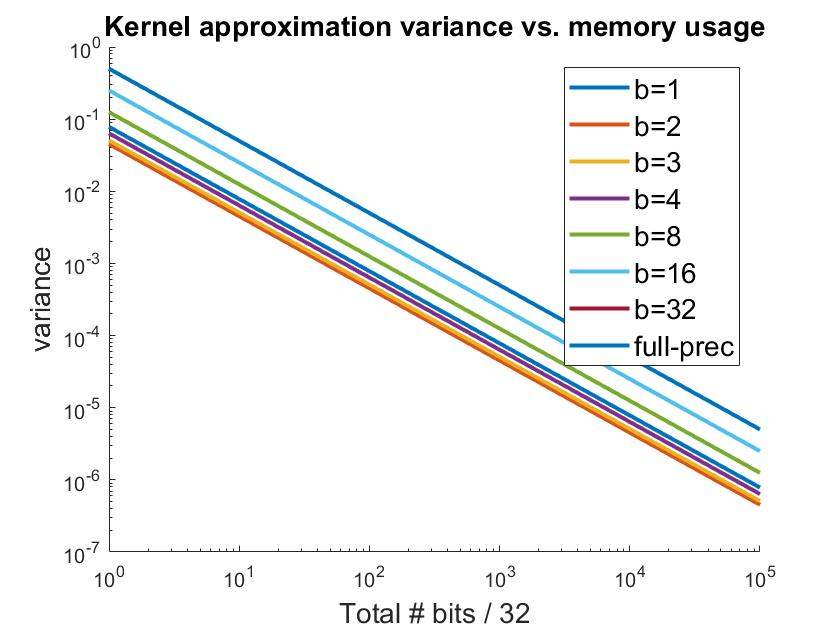
\includegraphics[width=0.6\textwidth]{lprff_variance_figure_numbits.jpg}
\end{center}
As you can see, lowering the precision helps reduce the variance by approximately a full order of magnitude ($10\times$ smaller variance) for a fixed number of bits, with $b=2$ giving the lowest variance, and $b=32$ variance matching the full-precision line (they are overlapping in the figure).  In the plot below, we show the kernel approximation variance as a function of the number of features.  As you can see, using $1$ bit per feature gives a noticeable jump in variance, but all other higher precision features perform comparably to the full-precision random features.

\begin{center}
	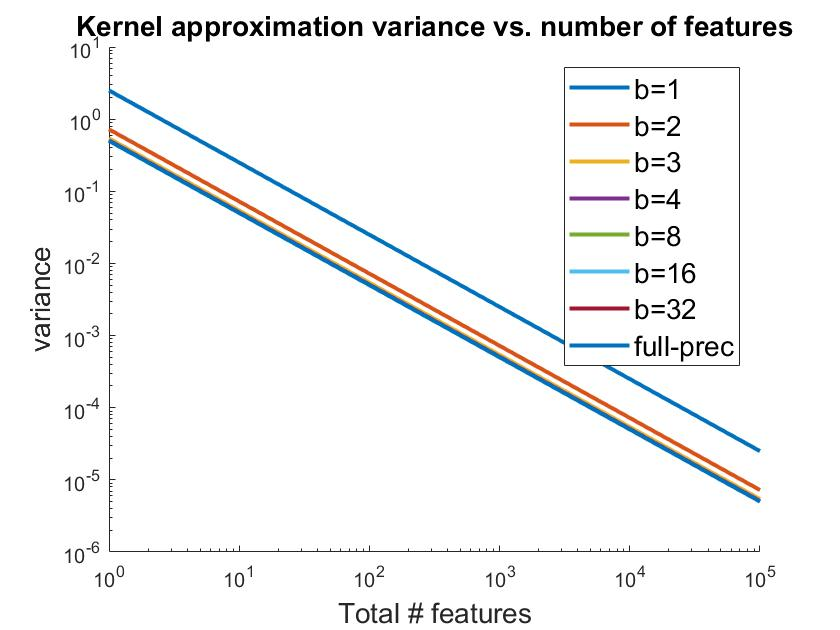
\includegraphics[width=0.6\textwidth]{lprff_variance_figure_numfeat.jpg}
\end{center}
% FIGURES
%figure; hold on;
%n = 1:100000;
%for b = [1,2,3,4,8,16,32]
%plot(n,(  (1/2) + 2/(2^(2*b)-2^(b+1)+1)  ) ./ n,'LineWidth',2)
%end
%plot(n,0.5./n,'LineWidth',2)
%lgd = legend('b=1','b=2','b=3','b=4','b=8','b=16','b=32','full-prec');
%lgd.FontSize = 14;
%xlabel('Total # features','FontSize',14)
%ylabel('variance','FontSize',14)
%title('Kernel approximation variance vs. number of features','FontSize',14)
%set(gca,'yscale','log')
%set(gca,'xscale','log')
%
%figure; hold on;
%n = 1:100000;
%for b = [1,2,3,4,8,16,32]
%plot(n,(  (1/2) + 2/(2^(2*b)-2^(b+1)+1)  ) ./ ((32/b) * n),'LineWidth',2)
%end
%plot(n,0.5./n,'LineWidth',2)
%lgd = legend('b=1','b=2','b=3','b=4','b=8','b=16','b=32','full-prec');
%lgd.FontSize = 14;
%xlabel('Total # bits / 32','FontSize',14)
%ylabel('variance','FontSize',14)
%title('Kernel approximation variance vs. memory usage','FontSize',14)
%set(gca,'yscale','log')
%set(gca,'xscale','log')
%



\item It is important to note that Propositions 2 and 3 hold as a function of the number of low-precision features, and \textit{match} the bounds for the \textit{same number} of high-precision features.\footnote{Some care is needed for Proposition 3, because the set of functions $\cF_p$ we are considering is different than the one in the original.  I believe I can show that for a properly defined set of quantization functions, our $\cF_p$ is a superset of the original, though I may need to update the constant $C$.}  This is pretty amazing!
\end{enumerate}

\subsection{Open Questions}
\begin{enumerate}
	\item Can we extend Claim 1 (Uniform convergence of Fourier features) from $[5]$ (Rahimi and Recht, 2007) to low-precision features $z(x)$, to prove that the probability that there exists $x,y\in\cX$ such that $|z(x)^Tz(y) -k(x,y)| \geq \eps$ is small?
	\item Can we perform training in such a way that the learned weights are also low-precision?  What guarantees can we get with a training algorithm of this form?
	\item How does the family of functions $\cF_p$ defined in Proposition 3 compare to the one in $[4]$ (Rahimi and Recht, 2008)?	
	\item What can we say about the spectrum of the low-precision features relative to the full-precision features, and the exact kernel?  Results here would allow us to apply the ``fixed design'' linear regression analysis (from my other notes) here.
	\item Can we use low-precision for $x$,$w$, and $b$ in the features $z(x) = \sq\cos(w^Tx+b)$?  What can we prove about this?
\end{enumerate}

\section{Motivation}
Random Fourier features are an effective way of scaling kernel methods to large datasets.  Unfortunately, this method often requires a very large number of features in order to attain strong performance.  For example, in my work in speech recognition, increasing the number of features from 100k to 400k continued to give meaningful improvements.  At this scale, the amount of memory and computation time required to train models becomes a big bottleneck. For example, the size of a GPU's global memory can limit the number of random features which can be used, if one would like to train the model fully on a single GPU.  

Furthermore, in my work comparing random Fourier features and the \Nystrom method, I observed that using \textit{many} random Fourier features allows for approximating a larger portion of the kernel's spectrum, which appears to be important for attaining strong performance. This is in contrast to the \Nystrom method, which under a similar computational budget, computes fewer more expensive features; although these features approximate the kernel matrix very well, they are inherently limited in how many of the kernel's eigenvalues they can approximate.  The take-away here appears to be: many cheap features is better than fewer expensive features, even if those expensive features approximate the kernel matrix very well.

In light of the computational bottleneck which arises when training models with very many random features, as well as the observation that using a large number of features is important for downstream performance (even if they have higher variance when approximating the kernel), I propose using \textit{low-precision} as a way to further scale these random feature methods.
Some challenges involved in implementing and analyzing this idea are as follows:

\begin{enumerate}
	\item What are the trade-offs in deciding the number of bits of precision which should be used for the data, the random projection matrix, the random features, and the model parameters?  Can we effectively learn models on single-bit random features?
	\item If the model is stored in low-precision, what optimization algorithm should be used during training in order to make this possible?
	\item Will the final model be low-precision or high-precision?  Another way of asking this is: Is low-precision a trick to speed up the training of a full-precision model (as in HALP), or will the entire system be low-precision at both train and test time?
	\item How can we formalize the way the additional noise caused by quantization will affect the training of the model?  Can we use variance reduction techniques like SVRG to deal with this, like in HALP?
	\item Can we somehow use this additional randomness in the feature generation process in order to generate ``error bars'' in the estimates of the trained model (\eg, by evaluating the model on several random draws of the randomly quantized features for the same data point, in order to produce a distribution of predictions)?
\end{enumerate}

I will now discuss a few ideas related to two aspects of this project: (1) computing the random features, and (2) training a model with these features.

\section{Computing the low-precision random features}
Here, I will discuss different ways of computing $\tz(x)$, the quantized version of $z(x) = \sqrt{\frac{2}{m}} \cos(W^T x + b) \in \RR^m$, where $x\in \RR^d$, $W\in \RR^{d\times m}$, $b \in \RR^m$, and $\cos(\cdot)$ is the element-wise cosine non-linearity. Note that below I will ignore the factor of $\sqrt{\frac{2}{m}}$, as it can be stored separately as the ``scale'' parameter $\delta$ of the $b$-bit low-precision representation $(\delta,b)$.
\begin{itemize}
	\item Compute $\cos(W^Tx + b)$ using full precision (where $W$ can be a structured random matrix to save time/space), and then quantize the output.
	\item First, quantize $x$, $W$, and $b$, as $\tx$, $\tW$, $\tb$.  Then, compute $\tW^T \tx + \tb$, pass this 
	through the cosine function, and quantize the output.
	\item Use low-precision floating point operations (eg, 16-bit) for all of the operations.
\end{itemize}
One important thing to note is that quantizing $x$,$W$, and $b$ in such a way that $\expect{\tx,\tW,\tb}{\tW^T\tx + \tb} = W^Tx+b$ does \textit{not} mean that $\expect{\tx,\tW,\tb}{\cos(\tW^T\tx + \tb)} = \cos(W^Tx + b)$.  Thus, features generated in this way would not necessarily produce unbiased estimates of the kernel function, which satisfy $\expect{}{z(x)^Tz(y)} = k(x,y)$.
For this reason, I think the first option above is likely the best path forward.

In the case of 1-bit random features, we could quantize as follows: Let $z_i'(x) = \cos(w_i^T x + b_i)$ be the unnormalized $i^{th}$ feature of $z(x)$, and let $\tz_i'(x)$ be its quantized version, which we are discussing.  
In order for $\expect{}{\tz_i'(x)} = z_i'(x)$, we could set $\tz_i'(x) = +1$ with probability $\frac{1 + z_i'(x)}{2}$, and $\tz_i'(x) = -1$ with probability $\frac{1 - z_i'(x)}{2}$.  Here, we were using $\tz_i'(x) \in \{-1,+1\}$.
Note that one can simulate storing a vector $x \in \{-1,+1\}^d$ as a binary vector $\hat{x}\in \{0,1\}^d$ by noticing that 
$\dotp{x,y}= 2 \dotp{\hat{x},\hat{y}} - d$.

\section{Training a model using low-precision random features}
In this section, we address the question of how to train a model using low-precision random features as input.  Essentially, this comes down to training a linear model on top of random features $\tz$ such that $\expect{}{\tz} = z$.  One potentially
great option is to use ``LM-HALP'', the version of HALP designed for learning linear models, presented as Algorithm 4 in the
recent submission.  One potential down-side to this approach is that it would mean that the learned model would be
full-precision, which may or may not be desirable (for example, computing the full-precision gradient over the entire dataset
could be prohibitively expensive, and perhaps even impossible in the case where the full-precision model doesn't fit in
memory).  Note that any of the options below which use low-precision for both train/test would be inherently limited in terms of
how close to the global optimum they could get, as discussed in the HALP paper.  Perhaps, however, the error introduced by this
quantization could be more than made-up for by the ability to learn a model in a higher-dimensional, more expressive, feature
space.  We present some alternative options to LM-HALP below:
\begin{itemize}
	\item \textbf{Perceptron updates}: We could use the perceptron algorithm for model updates, 
	which would ensure that all operations could be done in integer arithmetic.
	\item\textbf{ Quantized SGD updates (``LP-SGD'')}: Consider the full-precision SGD update of
	the form $w_{t+1} = w_t + g_t z_t$, where $z_t = z(x_t) \in \RR^m$ is the random
	feature representation corresponding to the randomly chosen training point $x_t$ at
	time $t$.  We could replace this update by updates of the form 
	$w_{t+1} = w_t + \tg_t \tz_t$, where $\expect{}{\tg_t} = g_t$, and $\tg_t$ is stored in
	low-precision format.  For example, in the case of logistic regression, 
	$g_t = \eta \big(y_t - p_t\big)$, where $y_t\in\{0,1\}$ is the label for $x_t$, $\eta \in \RR$ is the learning
	rate, and $p_t = p(Y_t=1|z_t,w_t) = (1+\exp(-w_t^Tz_t))^{-1}$.  So in the case where $y_t = 1$,
	$\tg_t$ could be equal to $1$ with probably $1-p_t$, and 0 otherwise; and in the case
	where $y_t = 0$, $\tg_t$ could be equal to $-1$ with probability $p_t$, and 0
	otherwise.  Here, I am assuming that $\eta$ is stored in the scale factor $\delta$
	of the low-precision format $(\delta,b)$ for $\tg_t$.	
	If $\tg_t$ is in $(\delta,b)$ low-precision format, and $\tz_t$ is in
	$(\delta',b')$ format, then $w_t$ would be in $(\delta\delta',b+b')$ format.
	Note also that computing $p_t$ requires using the $\exp(\cdot)$
	and $(\cdot)^{-1}$ operations, which would probably need to be done as floating point
	operations.
	\item \textbf{LP-SVRG}: We could directly use LP-SVRG.
	\item \textbf{Update dual variables instead of primal}: In terms of the dual variables $\alpha_i$, the
	model becomes $f(x) = \sum_{i=1}^n \alpha_i z(x_i)^T z(x)$. Letting 
	$Z\in \RR^{n\times m}$ be the matrix whose $i^{th}$ row is $z(x_i)$, this can be
	rewritten as $\alpha^T (Z z(x))$.  If the random features are binary, $Zz(x)$ 
	can be implemented very efficiently, and its output is an integer vector (note that for huge $Z$,
	this operation can be distributed across a cluster of machines).
	If $\alpha$ is stored in low-precision format (as it would be if updates of the form described above
	for perceptron or LP-SGD are used), this dot-product could be performed using low-precision
	integer arithmetic, which can also be implemented fast.  As far as updating the values of
	the dual parameters $\alpha_i$ during training, we can simply simulate the primal updates of the form 
	$w_{t+1} = w_t + \tg_t z_t$ by using $\alpha_t = \alpha_t + \tg_t$, where here I am using 
	$\alpha_t$ to denote the dual parameter corresponding to the random point $x_t$ chosen at time $t$.
	\item \textbf{Distributed optimization}: We could also consider large-scale distribution optimization algorithms (\eg, $[1,2]$) in order to speed up training.
\end{itemize}

\section{Kernel Approximation Variance Analysis for Low-Precision RFF}
\noindent\textbf{Definitions}: For $z \in [a,c]$, let $X_z^{a,c}$ be the random variable which with probability $\frac{z-a}{c-a}$ equals $c-z$, and with probability $\frac{c-z}{c-a}$ equals $a-z$. Furthermore, let $Q^{a,c}(z) = z + X_z^{a,c} \in \{a,c\}$ be the ``quantized'' version of $z$, corresponding to randomized rounding to $a$ or $c$.  The following lemmas are easy to verify:\\

\noindent\textbf{Lemma 1}: Using the definitions above, it follows that $\expect{}{X_z^{a,c}} = 0$, $\var{}{X_z^{a,c}} = (z-a)(c-z)$, $\expect{}{Q^{a,c}(z)} = z$, and $\var{}{Q^{a,c}(z)} = (z-a)(c-z)$.\footnote{Note that if $a=0$, $\var{}{X_z^{0,c}} = z(c-z)$, which is maximized at $z=c/2$, with variance $c^2/4$.  If $a=-c$, $\var{}{X_z^{-c,c}} = c^2-z^2$, which is maximized at $z=0$ with variance $c^2$.}\\

\noindent\textbf{Lemma 2}: Given $z,z' \in [-c,c]$, let $S = Q^{-c,c}(z)Q^{-c,c}(z')$.
Then $\expect{}{S} = zz'$ and $\var{}{S} = c^4-z^2z'^{2}$.\\
%and $\eps \sim X_z^{-c,c}$, $\eps' \sim X_{z'}^{-c,c}$, let $S = (z+\eps)(z'+\eps')$.  

\noindent \textbf{Lemma 3}:
Assume $z_x\sim Z_x, z_y\sim Z_y$, where
$z_x,z_y\in[-c,c]$, and $\expect{}{Z_xZ_y} = k(x,y)$, for some $x,y\in\cX$.\footnote{For example, one specific instance of the random variables $Z_x,Z_y$ is given by random Fourier features, where $z_x = \sq\cos(w^Tx+b),z_y = \sq\cos(w^Ty+b)$, $z_x,z_y\in[-\sq,\sq]$, for random $w,b$.}  Assume $\var{}{Z_xZ_y} = \sigma^2$, and let $\tsigma^2 = \var{}{Q^{-c,c}(z_x)Q^{-c,c}(z_y)} = c^4 - z_x^2z_y^2$.
Now, letting $T = Q^{-c,c}(Z_x)Q^{-c,c}(Z_y)$, it follows that $\expect{}{T} = k(x,y)$, and $\var{}{T} = \sigma^2 + \tsigma^2$. \\

\noindent\textbf{Proposition 1}: Let $S=Z_x Z_y$, $T = Q^{-c,c}(Z_x)Q^{-c,c}(Z_y)$, and $(S_1,\ldots,S_n)$, $(T_1,\ldots,T_n)$ be a random sequence of i.i.d. draws from $S$ and $T$ respectively.  Define $\bar{S}_n = \frac{1}{n}\sum_{i=1}^n S_i$, and $\bar{T}_n =  \frac{1}{n}\sum_{i=1}^n T_i$, to be the empirical mean of these draws.  It follows that $\expect{}{\bS_n} = \expect{}{\bT_n} = k(x,y)$, and that
$\var{}{\bS_n} = \frac{\sigma^2}{n}$, and $\var{}{\bT_n} = \frac{\sigma^2 + \tsigma^2}{n}$.\\

Now, let's analyze the variance of using $\bS_n$ to approximate $k(x,y)$, relative to $\bT_{n*(32/b)}$.  This corresponds to comparing the variance of using $n$ ``full precision''  features (which we will assume are 32-bit), relative to using $n*(32/b)$ $b$-bit low-precision features. Note that both of these feature representations use the same total number of bits.  We will in this case assume we are using random Fourier features, and thus that
$z_x,z_y \in [-\sq,\sq]$.  We will upper bound $\sigma^2$ in this context by $1$, given the results in $[3]$ for the RBF kernel.  Furthermore, it is important to note that the quantization noise $\tsigma^2$ is very much tied to the number of bits used to quantize the features $z_x$.  We will thus use $\tsigma_b^2$ to denote the variance introduced by quantizing into $b$-bits.  In this case, we divide the interval $[-\sq,\sq]$ into $2^b-1$ sub-intervals of equal size, and quantization is performed within each of these intervals; each interval is of size $r = \frac{2\sq}{2^b-1}$. 
Thus, from Lemma 1 (see footnote) the quantization error $\tsigma_b^2 \leq r^2/4 = \frac{2}{(2^b-1)^2}$.  This allows us to perform the comparison discussed above:

\begin{eqnarray*}
	\var{}{\bS_n} &=& \frac{\sigma^2}{n} \\
	&\leq& \frac{1}{n}. \\
	\var{}{\bT_{n*(32/b)}} &=& \frac{\sigma^2 + \tsigma_b^2}{n*(32/b)} \\
	&\leq& \frac{1 + \frac{2}{(2^b-1)^2}}{n*(32/b)}\\
	&=& \frac{b((2^b-1)^2 + 2)}{32n(2^b-1)^2}
\end{eqnarray*}

We now plot these two upper bounds on a log-log plot, for various values of $b$ and $n$.\\
\begin{center}
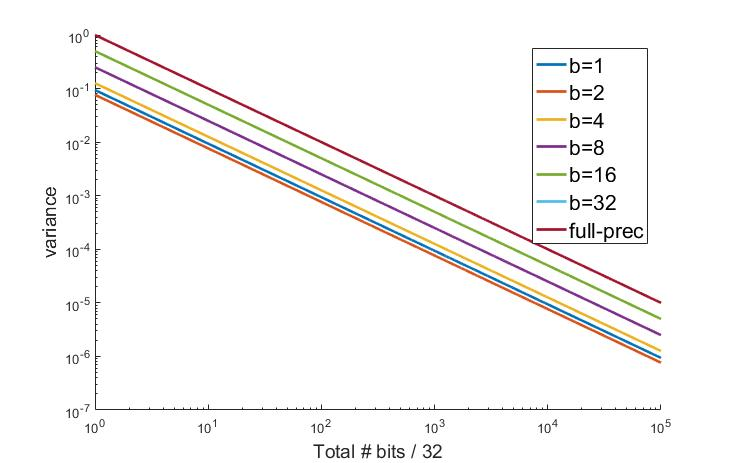
\includegraphics[width=0.6\textwidth]{lprff_variance_figure.jpg}
\end{center}
As you can see, lowering the precision helps reduce the variance by approximately a full order of magnitude ($10\times$ smaller variance), with $b=2$ giving the lowest variance, and $b=32$ variance matching the full-precision line (they are overlapping in the figure).

I will now discuss a concentration bound for these low-precision random features:\\
\textbf{Proposition 2}: For a fixed $x,y\in\cX$, let $S$ be any random variable with the property that $\expect{}{S} = k(x,y)$, and $S \in [-2,2]$.  Let $(S_1,\ldots,S_n)$, be a random sequence of i.i.d. draws from $S$, and let $\bS_n = \frac{1}{n}\sum_{i=1}^n S_i$ be the empirical mean of this sequence.  Then, it follows directly from Hoeffding's inequality that $\Prob{\big[|\bS_n - k(x,y)| \geq \epsilon\big]} \leq 2\exp(-n\eps^2/8)$.

\textbf{Open Question}: Can Claim 1 from Rahimi and Recht (2007) be adapted to this low-precision setting?  The most obvious obstacle here is that the randomness depends on the data; in other words, each $x \in \RR$ has a unique quantization noise distribution.  In other words, with the current definition, there is no way to draw all the random feature parameters upfront, in such a way that given these parameters, the feature functions are deterministic.  Can we somehow switch the quantization scheme for it to be deterministic?  For example, splitting the interval $[-\sq,\sq]$ into $r$ sub-intervals---then, for interval

\section{Generalization bounds for low-precision RFF}
We now discuss how to apply the result from Theorem 1 of Rahimi and Recht's 2008 paper to this low-precision setting [4].  That theorem assumes that there is a set of (deterministic) basis functions $\phi: \cX \times \Omega \rightarrow \RR$.  It then argues that if $\{w_1,\ldots,w_K\}$ are drawn independently from some distribution $p$ on $\Omega$, then the generalization performance of the model trained on the features $\phi(\;\cdot\;;w_i)$ is close to the best possible generalization performance of any model in the set $\cF_p = \{f(x) = \int_\Omega \alpha(w)\phi(x;w)dw | |\alpha(x)| \leq Cp(w)\}$.  Unfortunately, our randomly quantized features currently do not fit nicely into this framework, because the basis functions themselves are random, even for a fixed $x$ and $w$.  The purpose of the section below is to construct a parametrized set of basis functions $\phi(x;w,b,\theta)$ which quantize $\cos(w^Tx+b)$ in a deterministic way, given the parameters $\theta$.  This construction is a bit involved, but the goal is simple: 

We discuss how to deal with this below.
\subsection{Making random features ``deterministic''}
Let $\gamma > \eps_r > 0$ be two positive constants. Assume that we are using $b$ bits for our random features, and use these $b$ bits to express $2^b$ distinct values in the interval $[-(\sq + \gamma),\sq + \gamma]$.  If we divide the interval into $2^b - 1$ evenly sized intervals, each of size $\frac{2(\sq+\gamma)}{2^b - 1}$, this allows us to express the following set of values: $\frac{2(\sq+\gamma)}{2^b - 1}\cdot (-2^b + 1, -2^b + 3,\ldots, -1,1,\ldots, 2^b-3, 2^b -1)$.\footnote{Note that for simplicity here, I am dividing the entire interval into $2^b -1$ sub-intervals, which gives a symmetric set of $2^b$ positive and negative values expressible in $b$ bits, not including 0.  This differs from the presentation in the HALP paper, in which the set of expressible numbers is of the form $\delta\cdot (-2^{b-1}, \ldots, -1,0,1,\ldots,2^{b-1}-1)$.  We could use easily use the same notation as the HALP paper by using the values $\frac{2(\sq + \gamma)}{2^b-2}\cdot(-2^{b-1}, \ldots, -1,0,1,\ldots,2^{b-1}-1)$, though this ``wastes'' the smallest value $-\delta 2^{b-1}$ because it is smaller than $-(\sq + \gamma)$.}  We will call these intervals the ``quantization intervals'', whose boundaries correspond to the values expressible in $b$ bits.  Let $\hat{Q}_b$ denote this set of values.  Now, we will define another set of intervals, whose union will ``cover'' the set $[-\sq,\sq]$.  We will call these the ``rounding intervals'', and define them as follows.  Let $a$ be a uniformly at random ``offset'' chosen in the interval $[0,\eps_r]$.  Now, consider the following sequence of interval boundaries: $(-\sq-a,-\sq-a+\eps_r,-\sq-a+2\eps_r,\ldots,-\sq-a+R\eps_r)$, where $R=\ceil{(\frac{2\sq + a}{\eps_r})}$ is the smallest integer such that $-\sq-a+R\eps_r \geq \sq$.  Let $\hat{R}_a$ denote the set of boundary points for these rounding intervals, and let $c_k = \frac{1}{2}\Big((-\sq-a+(k-1)\eps_r) + (-\sq-a+k\eps_r)\Big)$ denote the center of the $k^{th}$ rounding interval.  For any value $z\in[-\sq,\sq]$, let $\ulq(z)$ be the ``bottom'' of the quantization interval containing $z$, let $\olq(z)$ denote the ``top'' of this interval, let $\ulr(z)$ be the ``bottom'' of the rounding interval containing $z$, let $\olr(z)$ denote the ``top'' of this interval, and let $c(z) =\frac{1}{2}(\olr(z) + \ulr(z))$  denote the center of this rounding interval.  Now, let $(X_1,\ldots,X_{R+1})$ denote $R+1$ Bernoulli random variables. The probability $p_k$ that
$X_k=1$ is defined as follows:
\begin{itemize}
	\item If the interval $[\ulr(c_k),\olr(c_k)]$ \textit{does not} contain one of the quantization boundaries:  
	$$p_k = \frac{c_k-\ulq(c_k)}{\olq(c_k)-\ulq(c_k)}.$$
	\item If the interval $[\ulr(c_k),\olr(c_k)]$ \textit{does} contain one of the quantization boundaries:  
	$$p_k = \frac{c_k-\ulq(\ulr(c_k))}{\olq(\olr(c_k))-\ulq(\ulr(c_k))}.$$
\end{itemize}
Let $k(z)$ denote the \textit{index} of the rounding interval in which $z$ falls: specifically, $k(z) = k' \Leftrightarrow z \in [-\sq-a+(k'-1)\eps_r, -\sq-a+k'\eps_r]$.  Now, if  $\theta=(\theta_1,\ldots,\theta_{R+1})$ are the outcomes of these $R+1$ Bernoullis, and $a$ is the random offset, we can define $g_{a,\theta}(z)$ as follows:
\begin{itemize}
	\item If the interval $[\ulr(z),\olr(z)]$ \textit{does not} contain one of the quantization boundaries:
	$$g_{a,\theta}(z) = (1-\theta_{k(z)})\ulq(z) + \theta_{k(z)}\olq(z).$$
	\item If the interval $[\ulr(z),\olr(z)]$ \textit{does} contain one of the quantization boundaries:
	$$g_{a,\theta}(z) = (1-\theta_{k(z)})\ulq(\ulr(z)) + \theta_{k(z)}\olq(\olr(z)).$$
\end{itemize}
Note that in the above definitions, even though the RHS does not contain $a$, it is implicitly dependent on $a$ through the $\olr$ and $\ulr$ functions.
Now, we are finally ready to define a set of ``deterministic'' basis functions:\footnote{I apologize for overloading the letter $b$ for both the number of bits, and the value in the expression $\cos(w^Tx+b)$.}
\begin{eqnarray*}
	\phi(x;w,b,a,\theta) &=&  g_{\theta,a}(\cos(w^Tx + b)). \\
\end{eqnarray*}

\textbf{Lemma 5}: If $z$ and $z'$ are in different rounding intervals, it follows that
\begin{eqnarray*}
zz' \leq \expect{a,\theta}{g_{a,\theta}(z)g_{a,\theta}(z')} \leq zz' + O(\eps_r).
\end{eqnarray*}

\textit{Proof}: We will first consider the case where $z$ is in the $k^{th}$ rounding interval $[\ulr(c_k),\olr(c_k)]$, and this interval \textit{does not} contain one of the quantization boundaries.  In this case, we will show that $\expect{\theta}{g_{a,\theta}(z)} = c_k$ (regardless of the value of $a$).  The case where the interval does contain a quantization boundary is very similar:
\begin{eqnarray*}
	\expect{\theta}{g_{a,\theta}(z)} &=&  \expect{\theta_k}{(1-\theta_k)\ulq(z) + \theta_k\olq(z)} \\
	&=& (1-p_k)\ulq(z) + p_k\olq(z) \\
	&=& \bigg(1-\frac{c_k-\ulq(c_k)}{\olq(c_k)-\ulq(c_k)}\bigg)\ulq(z) + \frac{c_k-\ulq(c_k)}{\olq(c_k)-\ulq(c_k)}\olq(z) \\
	&=& \frac{\olq(c_k)-c_k}{\olq(c_k)-\ulq(c_k)}\ulq(z) + \frac{c_k-\ulq(c_k)}{\olq(c_k)-\ulq(c_k)}\olq(z) \\
	&=& \frac{\olq(c_k)\ulq(z) - c_k\ulq(z) +c_k\olq(z) -\ulq(c_k)\olq(z)}{\olq(c_k)-\ulq(c_k)}\\
	&=& \frac{c_k\big(\olq(z)-\ulq(z)\big)}{\olq(c_k)-\ulq(c_k)}\\
	&=& c_k.
\end{eqnarray*}
In this sequence of equations, I used the fact that $\olq(z) = \olq(c_k)$, and $\ulq(z) = \ulq(c_k)$.

Now, I will use this fact to show that for $z$ and $z'$ in different rounding intervals ($k=k(z)$, $k'=k(z')$, $k\neq k'$), $\expect{a,\theta}{g_{a,\theta}(z)g_{a,\theta}(z')} = zz'$.

\begin{eqnarray*}
\expect{a,\theta}{g_{a,\theta}(z)g_{a,\theta}(z')} &=& 
\Exp_a \bigg[\Exp_{\theta}\big[g_{a,\theta}(z)g_{a,\theta}(z')\big] \bigg]   \\
&=& \Exp_a \bigg[\Exp_{\theta_k}\big[g_{a,\theta}(z)\big]  \Exp_{\theta_{k'}}\big[g_{a,\theta}(z')\big] \bigg]   \\
&=& \expect{a}{c_k c_{k'}}   \\
%\expect{a}{b}\expect{b}{f} \\
%&=& \int_{a=0}^{\eps_r} g_{a,\theta}(z)g_{a,\theta}(z')da\\
%&=& \int_{a=0}^{\eps_r} g_{a,\theta}(z)g_{a,\theta}(z')da %\sum_{(\theta_1,\ldots,\theta_{R+1})\in\{0,1\}^{R+1}}g_{a,\theta}(z)g_{a,\theta}(z')
\end{eqnarray*}

We can apply the above lemma as follows: Assume $x,y \in \cX$, and that $z_x = \sq \cos(w^Tx+b)$ and $z_y = \sq \cos(w^Ty+b)$.  It then follows from the lemma that:
\begin{eqnarray*}
\expect{w,b,a,\theta}{g_{a,\theta}(z_x)g_{a,\theta}(z_y)} &=& \expect{w,b}{z_x z_y} \\
&=& k(x,y)
\end{eqnarray*}

Thus, $\phi(x;w,b,a,\theta)\phi(y;w,b,a,\theta)$ is an unbiased estimate of $k(x,y)$ whenever
$z_x$ and $z_y$ are in different rounding intervals.

\section{Why 1-bit spectrum is terrible}
\begin{eqnarray*}
	A &=& XX^T \\
	&=& USU^T \\ %= \sum_i \lambda_i u_i u_i^T \\
	trace(A^T A) &=& trace( USU^T U S U^T)\\
	&=& trace( US^2 U^T) \\
	&=& \sum_i{\lambda_i^2}\\
	\tA &=& (X+C)(X+D)^T \\
	%	    &=& VTV^T \\
	\tA^T\tA &=& (X+D)(X+C)^T(X+C)(X+D)^T \\
	&=& XX^TXX^T + XC^TCX^T + DX^TXD^T + DC^TCD^T + \text{zero-mean}\\ 
	&=& A^TA + XC^TCX^T + DX^TXD^T + DC^TCD^T + \text{zero-mean}\\ 
	trace(\tA^T\tA) &=& trace(A^TA) + trace(XC^TCX^T) + trace(DX^TXD^T) + trace(DC^TCD^T) + trace(\text{zero-mean})\\ 
	&=& \sum_i \tilde{\lambda_i}^2\\
	\expect{}{\sum_i \tilde{\lambda_i}^2} &=& \expect{}{trace(\tA^T\tA)} \\
	&=& trace(A^TA) + \expect{}{trace(XC^TCX^T) + trace(DX^TXD^T) + trace(DC^TCD^T)} + \expect{}{trace(\text{zero-mean})}\\
	&=& trace(A^TA) + \expect{}{trace(XC^TCX^T) + trace(DX^TXD^T) + trace(DC^TCD^T)}\\	
	&\geq& trace(A^TA) \\
	&=&  \sum_i{\lambda_i^2} \\
	\expect{}{z^T \tA^T\tA z} &=& z^TA^TAz + \expect{}{z^T(XC^TCX^T + DX^TXD^T + DC^TCD^T)z} + \expect{}{z^T\text{zero-mean}z}\\ 
	&\geq& z^TA^TAz 
\end{eqnarray*}
So taking $z = u_i$, we get $\|\tA u_i\|^2 \geq \|Au_i\|^2 = \lambda_i^2$.
Can we show $\tA-A$ is PSD?

%(z_x+\teps_x)(z_y+\teps_y)$, where $\teps_x \sim X_{z_x}^{-\sq,\sq}$, and $\teps_y \sim X_{z_y}^{-\sq,\sq}$.
%Then $\var{}{\tS} = 4 - z_x^2 z_y^2$.
\section{References}
\noindent$[1]$ Large Scale Kernel Learning using Block Coordinate Descent.
Stephen Tu, Rebecca Roelofs, Shivaram Venkataraman, Benjamin Recht. \url{https://arxiv.org/pdf/1602.05310.pdf}. \\
$[2]$ CoCoA: A General Framework for Communication-Efficient Distributed Optimization.
Virginia Smith, Simone Forte, Chenxin Ma, Martin Takac, Michael I. Jordan, Martin Jaggi.  \url{https://arxiv.org/abs/1611.02189} \\
$[3]$ On the Error of Random Fourier Features. Dougal J. Sutherland, Jeff Schneider. UAI 2015. \url{https://arxiv.org/abs/1506.02785}\\
$[4]$ Weighted Sums of Random Kitchen Sinks: Replacing minimization with randomization in learning. Ali Rahimi, Ben Recht. NIPS 2008.\\
$[5]$	Random Features for Large-Scale Kernel Machines. Ali Rahimi, Benjamin Recht. NIPS 2007:
\end{document}
